 
 
\documentclass[crop,border={0pt 0 0 0},tikz]{standalone}
\usetikzlibrary{backgrounds,decorations.markings}
\tikzset{>=latex}
\tikzset{->-/.style={decoration={
  markings,
  mark=at position .5 with {\arrow{>}}},postaction={decorate}}}
\begin{document}
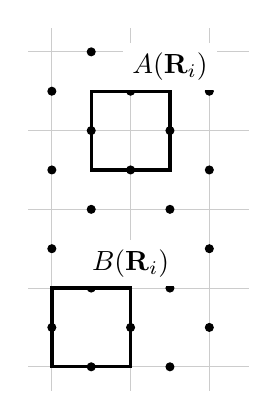
\begin{tikzpicture}
    
    \draw [step=1, line cap = rect, gray!40] (0.7,0.7) grid (3.5,5.3);
    
    \foreach \j in {1,...,4}
    { 
        \foreach \i in {1,...,2}
        {
            \draw[fill, xshift=0.5cm, yshift=0.5cm] (\i+0.5,\j) circle [radius=0.05];
            \draw[fill, xshift=0.5cm, yshift=0.5cm] (\i,\j+0.5) circle [radius=0.05];

        }
        
        % \draw[fill, xshift=0.5cm, yshift=0.5cm] (3.0,\j+0.5) circle [radius=0.05];
        % \draw[fill, xshift=0.5cm, yshift=0.5cm] (\j+0.5,3.0) circle [radius=0.05];
    }

    \foreach \j in {1,...,4}
    { 
            \draw[fill, xshift=0.5cm, yshift=0.5cm] (0.5,\j) circle [radius=0.05];
        
    }

    \foreach \j in {1,...,2}
    { 
            \draw[fill, xshift=0.5cm, yshift=0.5cm] (\j,0.5) circle [radius=0.05];
        
    }
    \draw[black, line cap=rect, very thick] (1.5,3.5) rectangle (2.5,4.5) node[anchor=south, fill = white] {$A(\textbf{R}_i)$};

    \draw[black, line cap=rect, very thick] (1,1) rectangle (2,2) node[anchor=south, fill = white] {$B(\textbf{R}_i)$};
    
    % \begin{scope}[shift={(7,0)}]
    %     \draw [step=1, line cap = rect, gray!40] (0.5,0.5) grid (3.5,3.5);
    
    % \foreach \i in {0,...,2}
    % { 
    %     \foreach \j in {0,...,2}
    %     {
    %         \draw[fill, xshift=0.5cm, yshift=0.5cm] (\i+0.5,\j) circle [radius=0.05];
    %         \draw[fill, xshift=0.5cm, yshift=0.5cm] (\i,\j+0.5) circle [radius=0.05];

    %     }
        
    %     \draw[fill, xshift=0.5cm, yshift=0.5cm] (3.0,\i+0.5) circle [radius=0.05];
    %     \draw[fill, xshift=0.5cm, yshift=0.5cm] (\i+0.5,3.0) circle [radius=0.05];
    % }

    % \draw[black, line cap=rect, very thick] (1,1) rectangle (2,2);
    % \end{scope}
\end{tikzpicture}
\end{document}
